%%
%% ****** ljmsamp.tex 13.06.2018 ******
%%
\documentclass[
11pt,%
tightenlines,%
twoside,%
onecolumn,%
nofloats,%
nobibnotes,%
nofootinbib,%
superscriptaddress,%
noshowpacs,%
centertags]%
{revtex4}
\usepackage{ljm}
\usepackage{listings}
\usepackage{xcolor}

\lstset{
language=C++,
basewidth=0.5em,
xleftmargin=45pt,
xrightmargin=45pt,
basicstyle=\small\ttfamily,
%keywordstyle=\bfseries\underbar,
keywordstyle=\color[rgb]{0,0,1},
numbers=left,
numberstyle=\tiny,
stepnumber=1,
numbersep=10pt,
showspaces=false,
showstringspaces=false,
showtabs=false,
frame=trBL,
tabsize=2,
captionpos=t,
breaklines=true,
breakatwhitespace=false,
escapeinside={\%*}{*)}
}

\begin{document}

\titlerunning{Vectorization} % for running heads
\authorrunning{Rybakov} % for running heads
%\authorrunning{First-Author, Second-Author} % for running heads

\title{Vectorization of the integer calculations \\ in the graph decomposition problem}
% Splitting into lines is performed by the command \\
% The title is written in accordance with the rules of capitalization.

\author{\firstname{A.~A.}~\surname{Rybakov}}
\email[E-mail: ]{rybakov.aax@gmail.com,rybakov_aan@nrcki.ru,rybakov@jscc.ru}
\affiliation{National Research Centre \textquotedblleft Kurchatov Institute\textquotedblright, 123182, Moscow, Academician Kurchatov sq. 1, Russia.}

%\author{\firstname{B.}~\surname{Second-Author}}
%\email[E-mail: ]{Second.Author@email.com}
%\affiliation{Place of work and/or the address of the first and second authors}
%\affiliation{Place of work and/or the address of second authors}
%\noaffiliation % If the author does not specify a place of work.

\firstcollaboration{(Submitted by TODO)} % Add if you know submitter.
%\lastcollaboration{ }

%\received{June 13, 2018} % The date of receipt to the editor, i.e. December 06, 2017

\begin{abstract} % You shouldn't use formulas and citations in the abstract.
The article is devoted to the problem of integer calculations vectorization.
Integer calculations is a program context which mainly works with integers and contains a large number of control transfer operations.
Such a program context is often found in combinatorial optimization problems where one has to work with discrete data structures, memory access indirection, and loop nests with an irregular number of iterations.
These factors negatively affect the use of vectorization, and automatic vectorization is almost impossible for such a context.
The article discusses the possibility of using the AVX-512 instructions set to vectorize code with the listed features, since the advantages of masked vector operations make it possible to achieve acceleration even in the presence of such bottlenecks.
The application of vectorization is considered using the example of a bubble growth algorithm for graph decomposition, where the graph is represented as lists of vertex adjacencies.
For the algorithm under consideration, a method is described for applying vectorization to loop nests using integer masked vector instructions from the AVX-512F set.
The vectorized decomposition algorithm has been tested on graphs with up to 4 million vertices.
Practical results were obtained on an Intel Xeon Phi 7290 Knights Landing microprocessor, and they demonstrated acceleration of the program code in the range of 1.7 -- 2.2 times, depending on the size of the computational mesh.
\end{abstract}

\subclass{68W10, 68R10} % Enter 2010 Mathematics Subject Classification.

\keywords{vectorization, AVX-512, integer calculations, combinatorial optimization, graph decomposition, bubble growth algorithm} % Include keywords separeted by comma.

\maketitle

% Text of article starts here.

\section{Introduction}

High-performance computing makes it possible to simulate natural and technological processes with a high degree of detail, simultaneously take into account many factors of various origins, and quickly analyze numerous options.
This allows us to obtain a picture of the process under study with the required accuracy, reflecting the actual situation as much as possible instead of expensive, dangerous or even impossible full-scale experiments.
The use of supercomputing technologies can significantly reduce the cost and time required to create new competitive products, facilities, and systems.
The range of high-performance computing applications is very wide.
Thus, using supercomputer modeling, problems of gas dynamics and hydrodynamics \cite{01Smirnov}, molecular dynamics \cite{02Guo}, plasma physics \cite{03Asch}, solid mechanics \cite{04Morgan}, mathematics \cite{05Lohiya} and others are solved.
High-performance computing is used to solve such large computational scientific and technical problems as atmospheric modeling \cite{06Kang}, aircraft design \cite{07Morad}, exploration of oil and gas fields \cite{08Eremin}, modeling of large molecules and polyatomic systems \cite{09Yan} and many others.

When solving a computational problem on a supercomputer system, parallelization must be performed between its nodes to speed up calculations \cite{10Voevodin}.
The next level of computing parallelization is parallelization within a single computing node on shared memory \cite{11Zhou}.
The lowest level of calculations parallelization can be considered vectorization -- parallelization at the level of individual instructions \cite{12Feng}.

Vectorization is an important low-level optimization of software code, which can be used to achieve multiple acceleration of supercomputer applications.
All major modern microprocessor architectures (x86, ARM, Power, <<Elbrus>>, LoongArch, Sunway, and others) support vector computing, and there is a tendency to increase the size of the vector (today the maximum length is 512 bits, but now this length is logically unlimited, given the sets of vector instructions with a variable length of the vector).

Currently, the most advantageous set of vector instructions is the AVX-512, as it supports the possibility of selective processing of vector elements using vector masks.
This unique feature allows to vectorize a complex programming context containing control transfer commands, loop nests, and function calls.
It can be considered that for the first time the AVX-512 vector instructions set was supported in 2016 in Intel Xeon Phi Knights Landing (KNL) microprocessors, since the earlier generation Intel Xeon Phi Knights Corner (KNC) was an accelerator, and the vector code for it is not x86 compatible.
Since that moment, the issues of application vectorization have been actively discussed in the scientific community.
There are many papers on the vectorization of the software in application to various subject areas: gas dynamic solvers \cite{12-1Kulikov}, encryption tools \cite{12-2Buhrow}, time series analysis \cite{12-3Quislant}, sorting of an array of numbers \cite{12-4Blacher}, fast Fourier transform \cite{12-5Sansone} and more.

In this paper, we will consider the application of vectorization using the AVX-512 instruction set to integer calculations containing loops with an irregular number of iterations.
As such, we will take the bubble growth algorithm of graph decomposition, in which a simultaneous breadth-first traversal of the graph is performed from randomly located initiating vertices.

\section{Bubble growth graph decomposition algorithm}

Currently, there is a wide variety of graph decomposition algorithms that are applied depending on the size of the graph being processed and the requirements for the quality of decomposition \cite{13Ayall}.
At the same time, the size requirements of the processed graphs are constantly increasing, and today the decomposition problem is considered for graphs containing tens of millions of vertices or more \cite{14Lee}.
When performing graph processing, the main operation is to obtain incident edges and neighboring vertices of a given vertex.
The way this action is performed depends on the internal representation of the graph in the computer memory \cite{15Ahmed,16Salwasser}.
We will consider a representation of an undirected graph in which a list of neighboring vertices is available for each vertex index.
Let's consider the following graph decomposition algorithm -- the bubble growth algorithm -- which is one of the simplest in terms of work logic.

\begin{figure}[h]
\setcaptionmargin{5mm}
%\onelinecaptionsfalse % if the caption is multiline
\onelinecaptionstrue  % if the caption is one-line
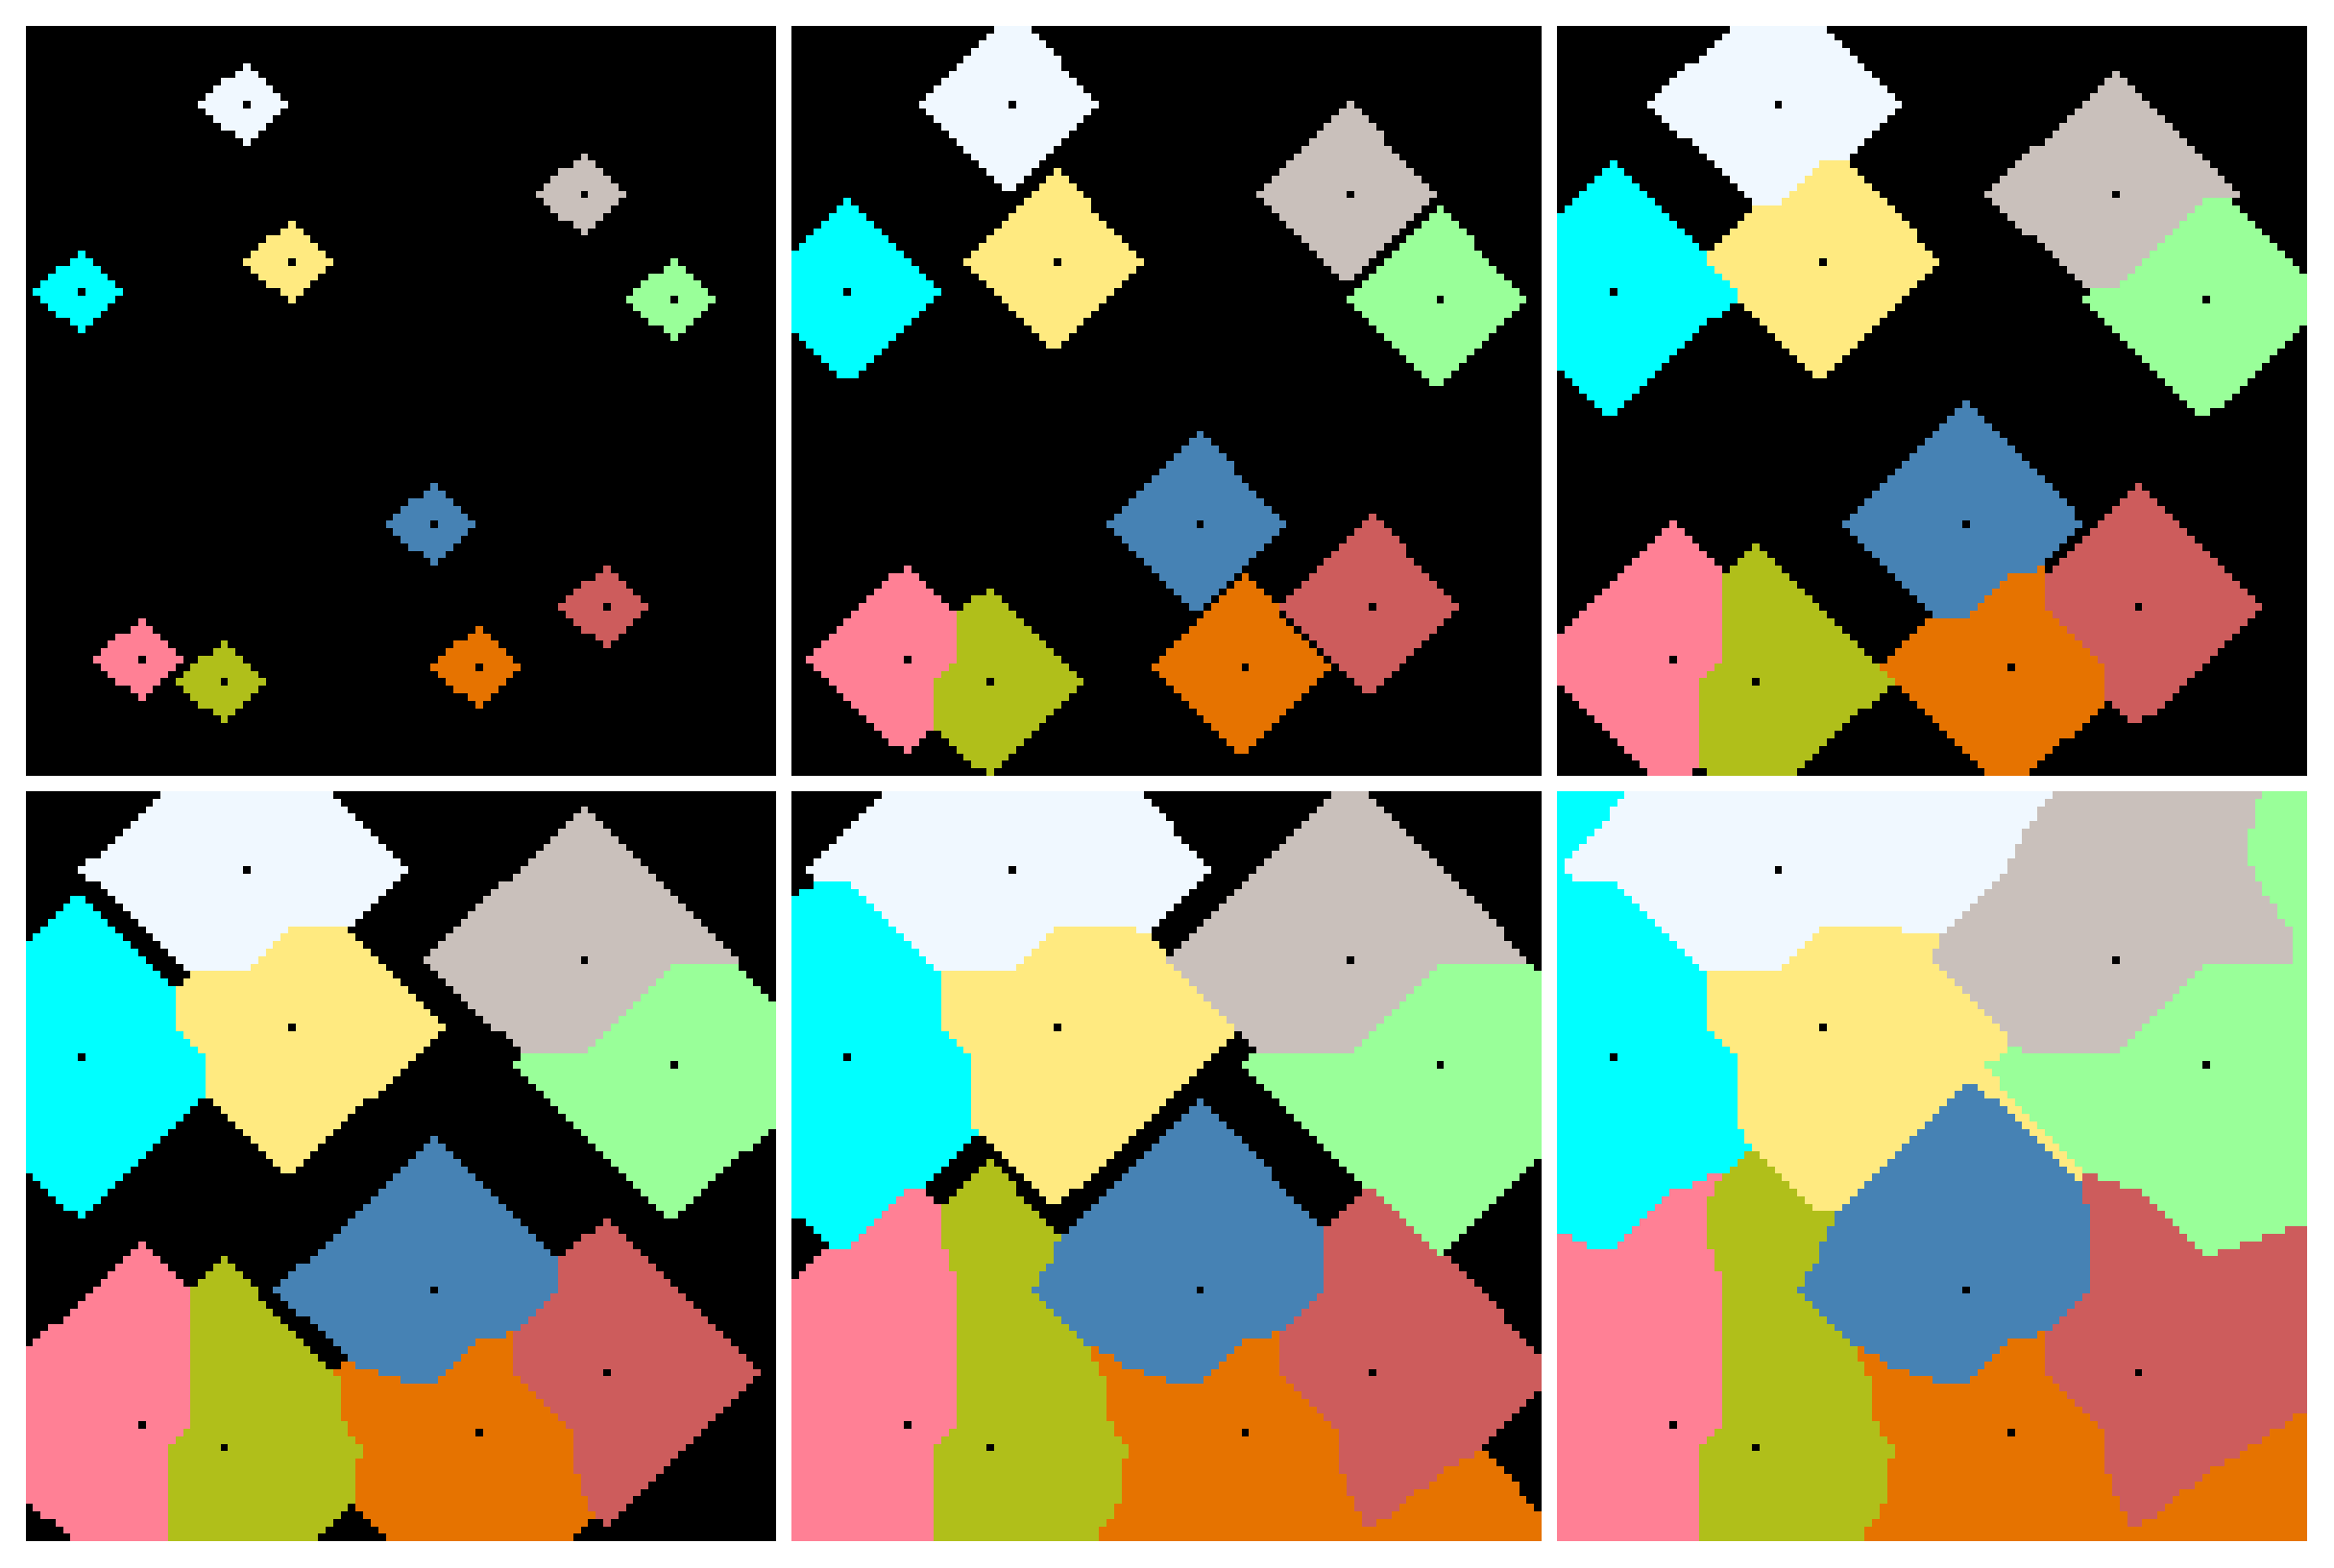
\includegraphics[width=0.65\textwidth]{pics/incr.pdf}
\captionstyle{normal}\caption{Domain growth during the bubble decomposition algorithm.}\label{fig:incr}
\end{figure}

The bubble growth algorithm for graph decomposition \cite{17Fan} is based on a breadth-first traversal of the graph, performed simultaneously, starting from several initiating vertices.
At the beginning of the algorithm, the initiating vertices are randomly selected (according to the required number of domains).
Each of the selected vertices belongs to a corresponding domain.
After that, the process of simultaneous domains building begins.
At each iteration of the algorithm, each domain is increased by one vertex that has not yet been assigned to any domain (if this can be done).
The process ends when all the vertices of the graph are distributed across domains.
Fig.~\ref{fig:incr} illustrates the process of building domains from randomly selected vertices for a graph on a plane.

After distributing all the vertices by domain, its center is calculated for each domain, after which the domain centers are taken as new initiating vertices, the graph decomposition is reset, and then the domains are built from these new initiating vertices.
This process can continue either a fixed number of times, or until a certain condition is reached (stabilization of the initiating vertices, achieving a balanced partition, repeating the previously obtained configuration) \cite{18Golovchenko}.
The bubble growth algorithm does not guarantee a balanced division into domains or the formation of short boundaries between domains.
However, this algorithm is distinguished by its simplicity, which allows it to be used as a basic operation in complex approaches to the graph decomposition \cite{19Wu}.

Let us briefly note the potential of using the bubble growth algorithm in the family of genetic algorithms \cite{20Katosh}.
Genetic algorithms are nature-like heuristic algorithms that are actively used to solve optimization problems with a large number of parameters \cite{21Wirayanti}.
During the operation of the genetic algorithm, the survival process of a population consisting of individual individuals is modeled, each of which represents a solution to some optimization problem.
To implement the algorithm, the concept of a genotype (some code of an individual) must be defined, the process of creating an individual based on its genotype must be implemented, the fitness function of the individual must be determined, and the operations of crossing and mutating individuals at the genotype level must be implemented.
In the process of population evolution, the weakest individuals die out, while the more fit ones leave offspring, which leads to an increase in the average value of the fitness function of individuals in the population.
Genetic algorithms are applicable for solving combinatorial optimization problems, in particular for graph decomposition problems.
However, when using a genetic algorithm to solve the graph decomposition problem, the concepts of genotype and individual are often mixed.
For example, in \cite{22Chaouche}, when decomposing a graph, each edge is encoded in the genotype, and in \cite{23Li}, the explicit distribution of vertices across domains is encoded in the genotype.
In other words, the genotype practically replaces the concept of an individual, which leads to a significant slowdown in the work of the genetic algorithm and the impossibility of its use for the decomposition of large graphs.
Also, the application of the mechanisms of crossing and mutation directly to individuals is questionable from the point of view of correctness.
The simplicity and speed of the bubble growth algorithm allows it to be used in genetic algorithms as an operation for constructing an individual from a genotype represented by a set of initiating vertices.
In this case, the shift of the initiating vertex to a random neighbor can be considered as a genotype mutation.
This approach of using the bubble growth algorithm inside the genetic algorithm has been approbated in practice, and the solution is available in an open repository https://github.com/r-aax/mendel.

\section{Bubble growth algorithm vectorization}

The use of the bubble growth algorithm as a single operation in complex approaches to graph decomposition (like the genetic algorithm) places increased demands on its performance.
Let's consider the possibilities of speeding up this algorithm using AVX-512 instructions set for vectorization.
Let's say we have a graph, information about its edges is written in the structure \texttt{vector$<$vector$<$int$>>$ inc}, where \texttt{inc[i]} is a list of numbers of all vertices adjacent to the vertex \texttt{i} (adjacency list, or vertex neighborhood).
The domain numbers that specific vertices belong to are stored in the \texttt{vector$<$int$>$ domains} structure.
The \texttt{vector$<$queue$<$int$>>$ q} structure is a list of queues.
Each queue \texttt{q[i]} is queue of vertices waiting to enter \texttt{i}-th domain.
At the beginning of the algorithm, the \texttt{q[i]} queue contains only one initiating vertex of the \texttt{i}-th domain.
Let's say we need to decompose the graph (or color the graph) into \texttt{domains\_count} domains.
Then the simple implementation of the bubble growth algorithm for domains from the initiating vertices may be written as simultaneous breadth-first traversal of the graph starting from the initiating vertices (see Listing~\ref{lst:impl}):

\begin{lstlisting}[caption={Implementation of the bubble domain growth algorithm.},label={lst:impl}]
while (is_q)
{
    is_q = false;

    for (size_t c = 0; c < domains_count; ++c)
    {
        if (q[c].empty()) continue;

        is_q = true;
        n = q[c].front();
        q[c].pop();

        if (domains[n] == -1)
        {
            domains[n] = c;
            for (auto ngh : inc[n]) q[c].push(ngh);
        }
    }
}
\end{lstlisting}

The implementation of the algorithm is performed as the nest of 3 loops.
The outer loop is executed until there is at least one non-empty domain queue (that is, there are vertices not allocated by domains).
The middle cycle is performed by domain numbers.
For each domain, the first vertex is taken from the corresponding queue, and if it has not yet been assigned to any domain, it is entered into the current domain, and all its neighbors are sent to the queue.
The inner loop is a loop through all the neighbors of the newly processed vertex that should be queued.
We will perform vectorization of the presented code by the middle cycle, and for ease of analysis, we will provide an implementation for a fixed value \texttt{domains\_count = 16} (this will get rid of the middle cycle and replace it with a set of separate vector operations).

To perform vectorization, we first need to get rid of the STL structures (\texttt{vector} and \texttt{queue}), since they have their own internal implementation, and vectorization of operations for working with them is impossible.
Instead of the \texttt{vector$<$int$>$} structure, we will store information about the list of neighboring vertices simply in an array, the 0-th element of which will be its size.
The queue will also be simulated using an array and indexes \texttt{front} and \texttt{back}, pointing to the first and last elements of the queue, respectively.
Then the operation \texttt{push(v)} will correspond to writing into the array at the index \texttt{back} with its incrementation, and the operation \texttt{pop} will correspond simply to the incrementation of the index \texttt{front}.
The queue is empty if its index \texttt{front} is greater than the index \texttt{back}.

\begin{figure}[h]
\setcaptionmargin{5mm}
\onelinecaptionsfalse % if the caption is multiline
%\onelinecaptionstrue  % if the caption is one-line
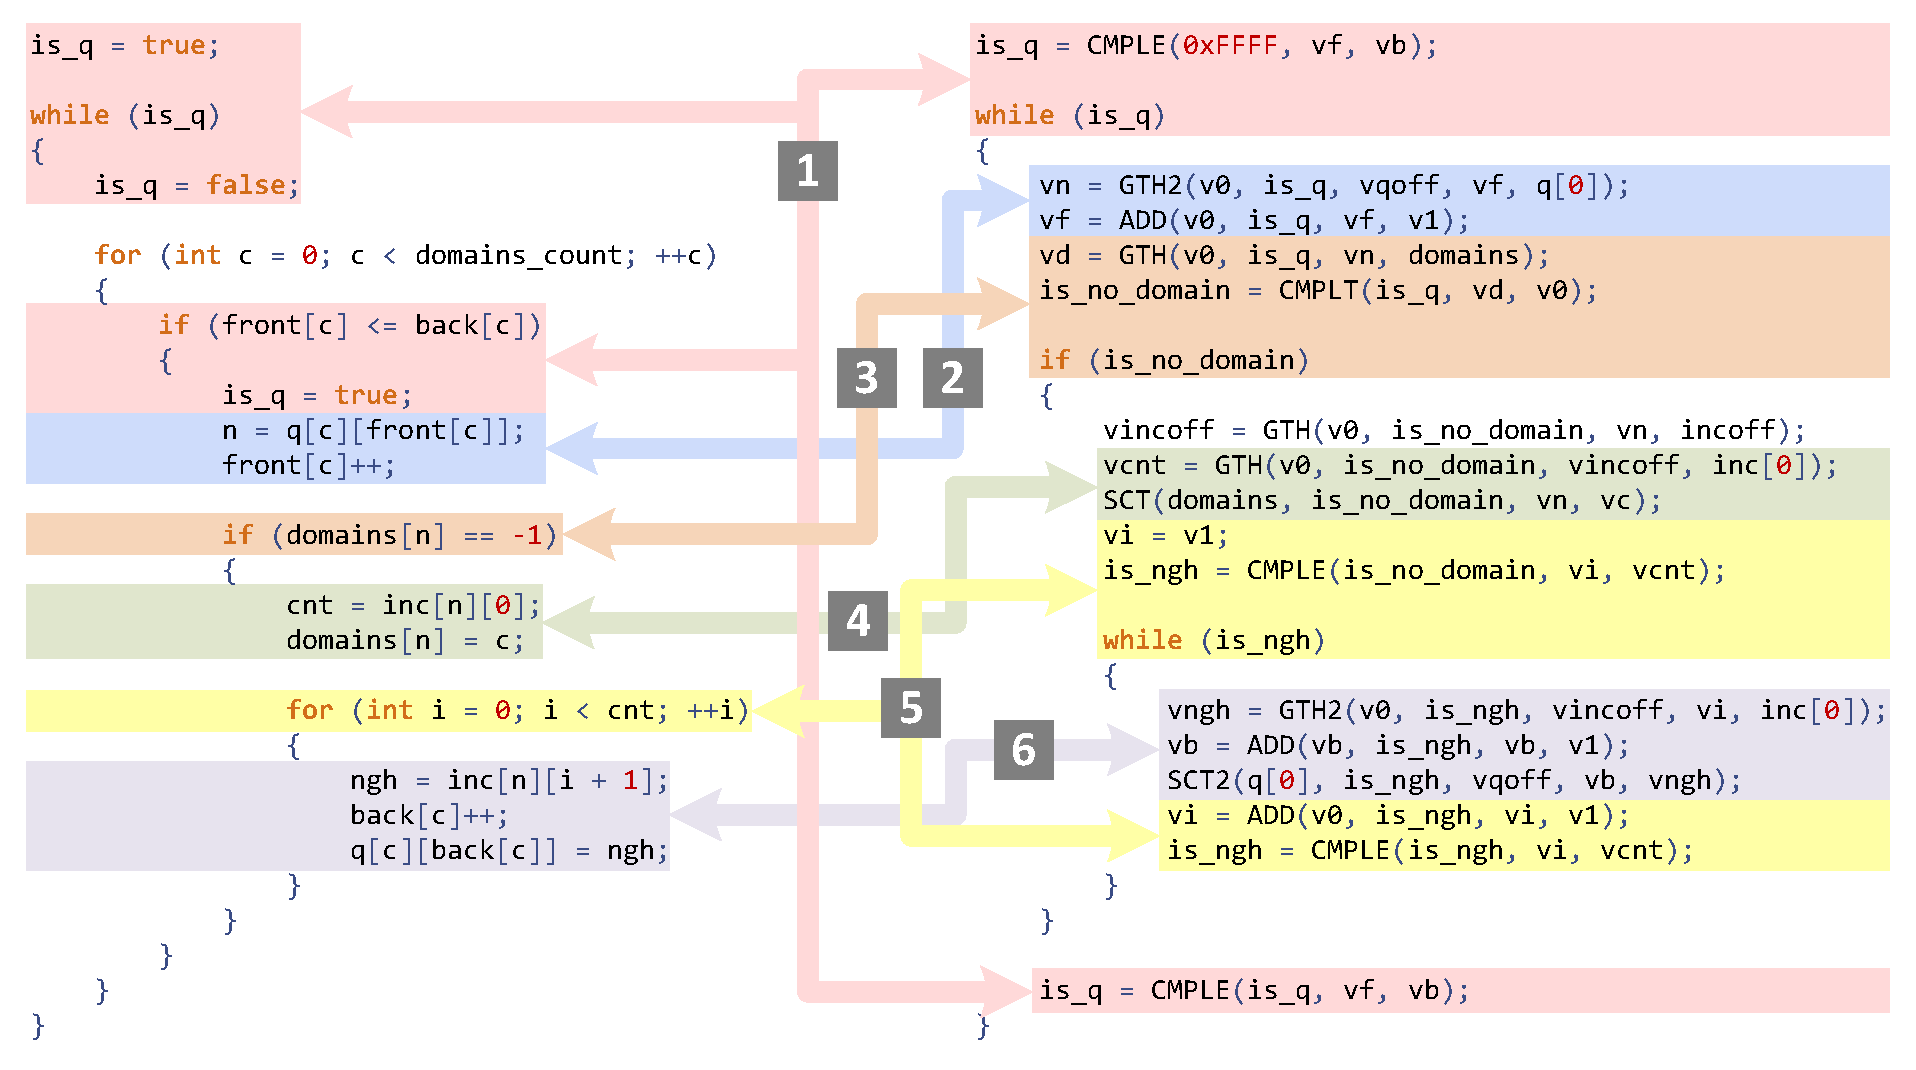
\includegraphics[width=0.85\textwidth]{pics/code.pdf}
\captionstyle{normal}\caption{Vectorization of the bubble growth algorithm program code by replacing scalar instructions with vector analogues.}\label{fig:code}
\end{figure}

On Fig.~\ref{fig:code} the scalar and vector versions of the software code for implementing the bubble growth algorithm are presented.
In the vector version, \texttt{ADD}, \texttt{GTH}, \texttt{SCT} are used to denote the intrinsic functions \texttt{\_mm512\_mask\_add\_epi32}, \texttt{\_mm512\_mask\_i32gather\_epi32}, \texttt{\_mm512\_i32scatter\_epi32} respectively (\texttt{GTH2} and \texttt{SCT2} are the same operations \texttt{GTH} and \texttt{SCT}, only using two offsets from the base address at once).
Using \texttt{CMPLE}, \texttt{CMPLT}, the calls to the intrinsic function \texttt{\_mm512\_mask\_cmp\_epi32\_mask} are indicated with the comparison parameters \texttt{\_MM\_CMPINT\_LE} and \texttt{\_MM\_CMPINT\_LT}, respectively.
On Fig.~\ref{fig:code} the digit <<1>> indicates the vectorization of the condition for continuing execution of the outer loop (the loop terminates if all domain queues are empty).
The number <<2>> indicates the vectorization of extracting the next vertex from each queue.
The number <<3>> indicates that the extracted vertices belong to a domain (in the vector version, a mask \texttt{is\_no\_domain} is formed -- a mask with the numbers of the domains to which the new vertex is added).
The number <<4>> indicates the vectorization of placing the vertex into the current domain and obtaining the number of its neighbors.
The digit <<5>> is processing all the neighbors of the vertex just placed in the domain, and the digit <<6>> is adding these neighbors to the corresponding queues.

It is worth noting that the vectorized version of the presented algorithm is not fully equivalent to the scalar version.
It may well turn out that at some iteration of the outer loop, the same vertex will be extracted from two or more different queues at the same time.
In this case, in the vector version, it will be assigned to the domain with the highest number (although in the scalar equivalent, it would fall into the domain with the lowest number).
This discrepancy can be eliminated by turning around the vectors \texttt{vn} and \texttt{vc} when writing to the array \texttt{domains} (digit <<4>> on Fig.~\ref{fig:code}), but this operation was not implemented for code simplification.

\begin{figure}[h]
\setcaptionmargin{5mm}
\onelinecaptionsfalse % if the caption is multiline
%\onelinecaptionstrue  % if the caption is one-line
\begin{tabular}{ll}
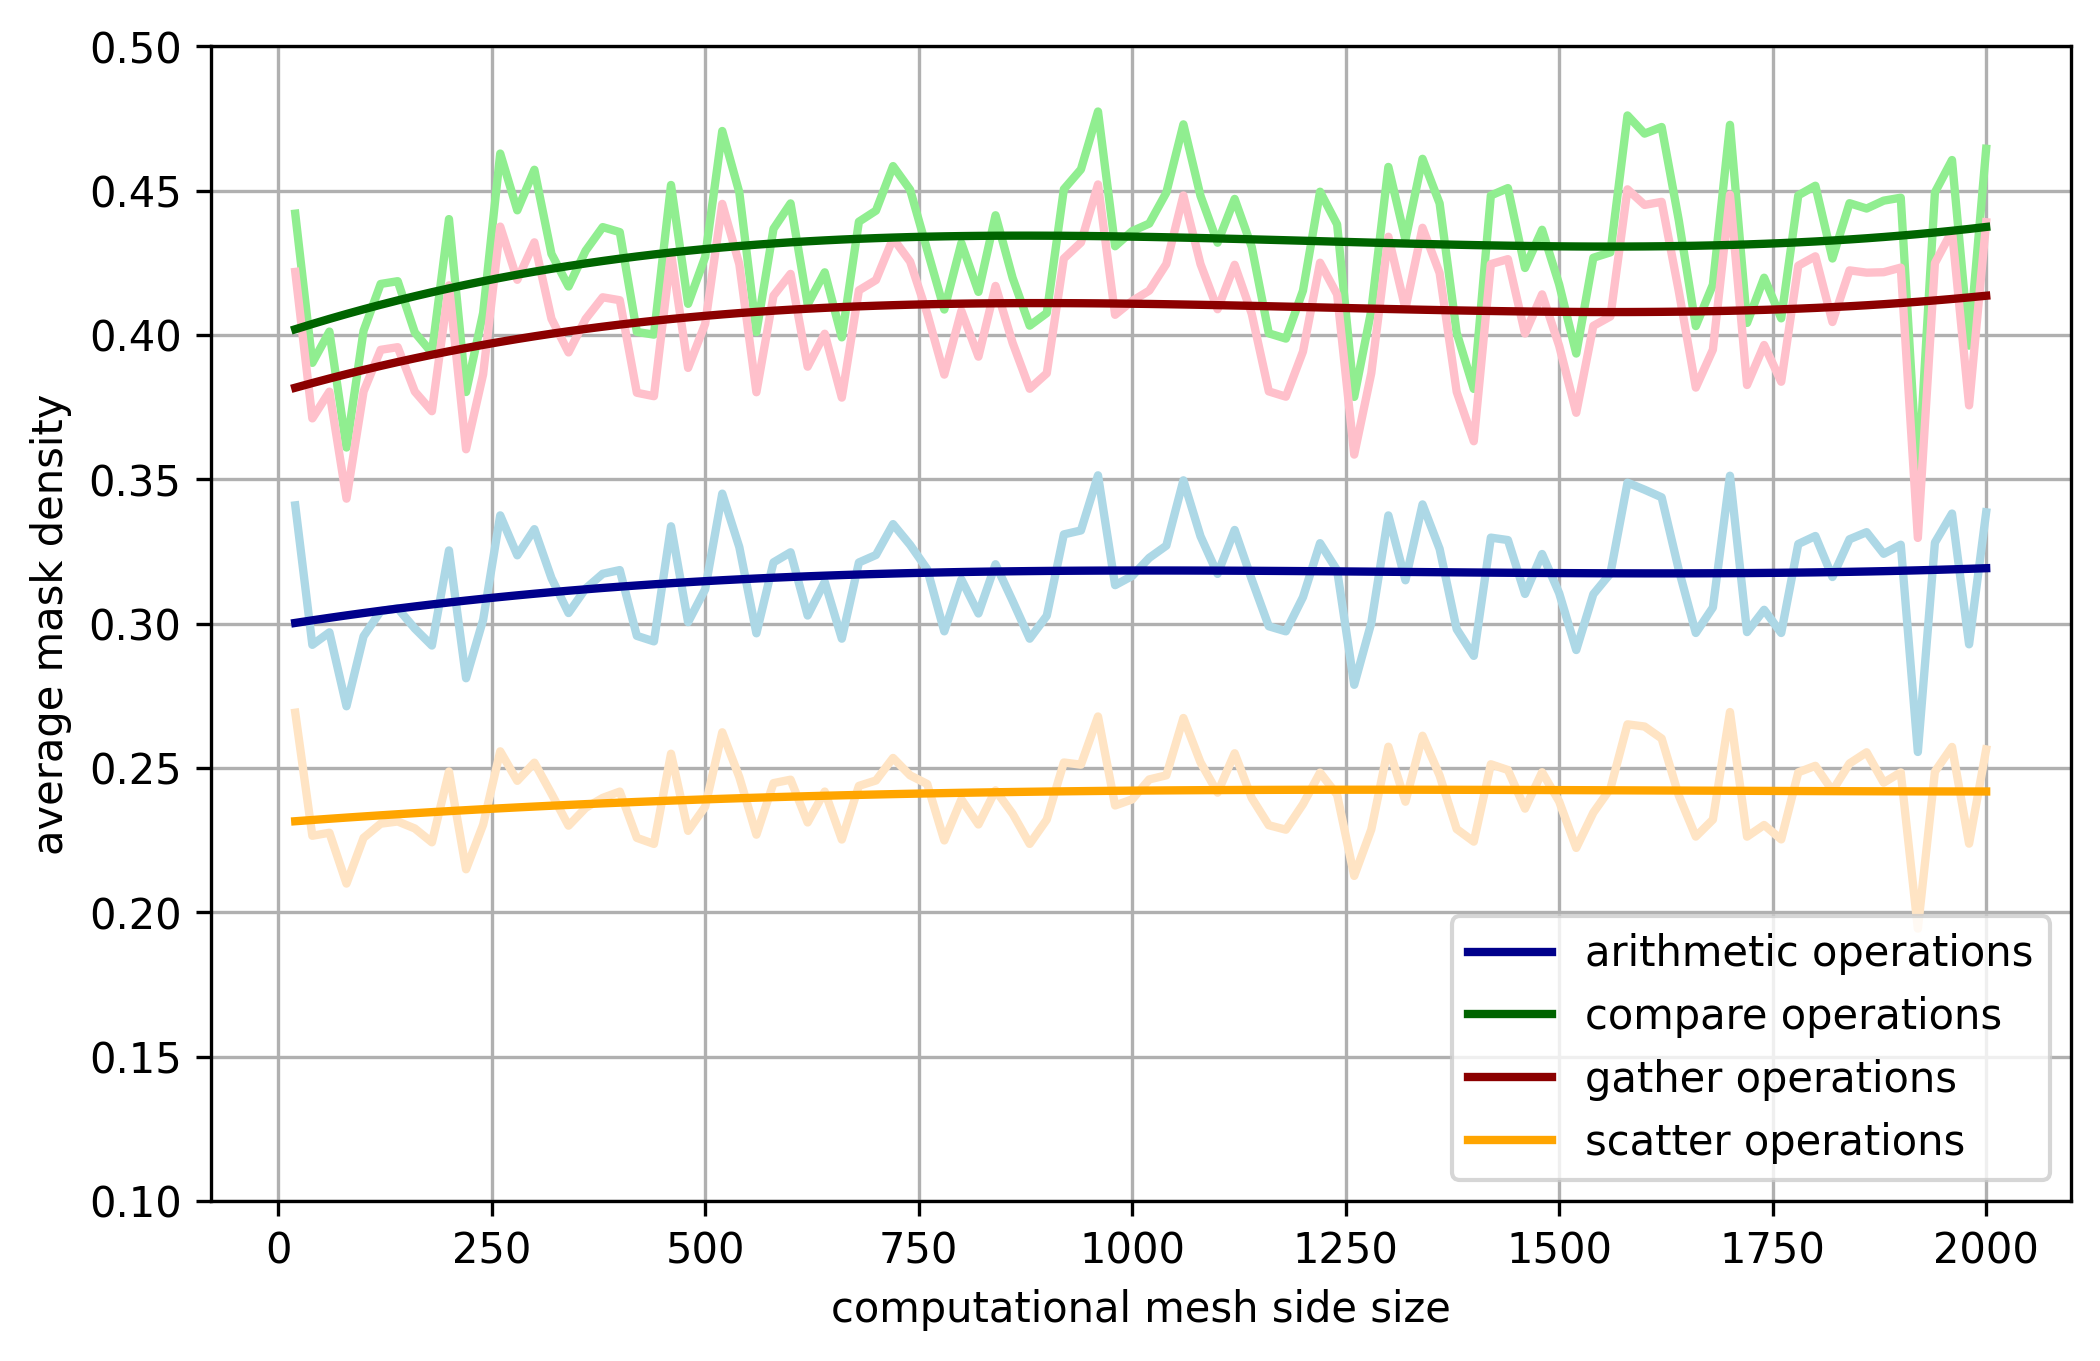
\includegraphics[width=0.45\textwidth]{pics/chart_statistics_eng.png}
&
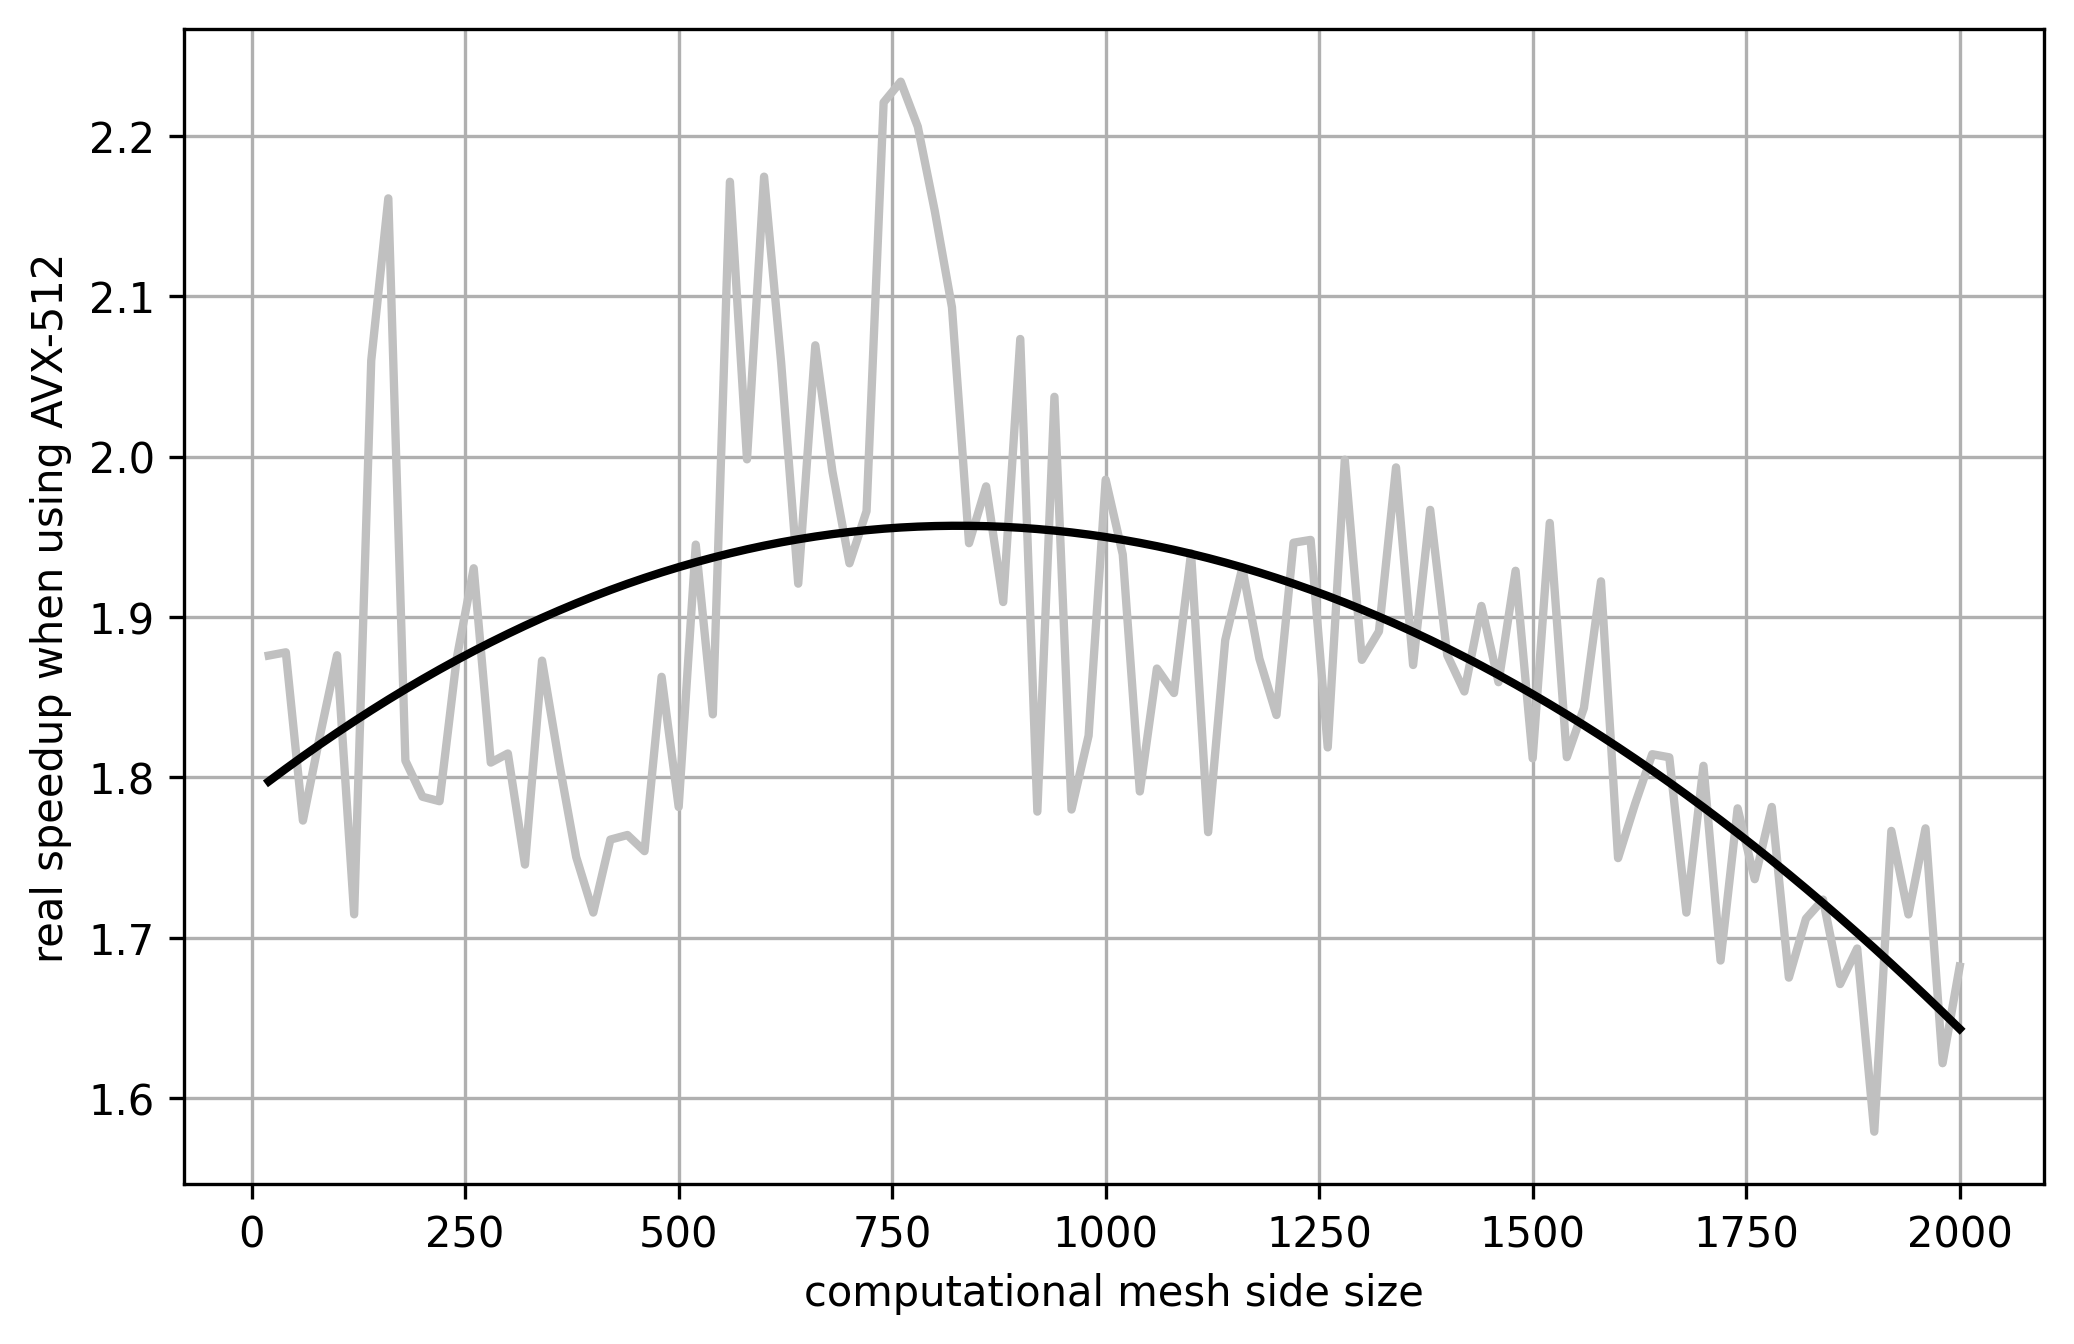
\includegraphics[width=0.45\textwidth]{pics/chart_speedup_eng.png}
\end{tabular}
\captionstyle{normal}\caption{The average density of masks for different AVX-512 operations classes (on the left) and the acceleration of calculations obtained on Intel Xeon Phi 7290 Knights Landing (on the right).}\label{fig:chart}
\end{figure}

To evaluate the effectiveness of the vectorization, test runs were performed for dual graphs of surface rectangular computational meshes with sides from 20 to 2000 cells (that is, on graphs with a number of vertices from 400 to 4 million).
On Fig.~\ref{fig:chart} on the left is the collected statistics on the masks density (fraction of set bits) of various operations types.
From these charts, we can immediately conclude that vectorization is not very efficient, since the density of masks for arithmetic operations and write operations to memory turned out to be quite low (about 0.3 and 0.25, respectively).

Measurements of the actual acceleration were performed for the same graphs on an Intel Xeon Phi 7290 Knights Landing microprocessor, the results are shown on Fig.~\ref{fig:chart} on the right.
For convenience, there is also a chart of the smoothed acceleration indicator.
Analyzing the chart of the smoothed acceleration indicator, it can be noted that the maximum is observed when the side of the computational mesh is around 750 and is approximately 1.95.
The decrease in acceleration when reducing the side of the computational mesh is associated with an increase in the number of conflicts when processing the next vertices from the domain queues.
The decrease in acceleration with an increase in the side of the computational mesh is associated with an increase in the spread of offsets when performing gather/scatter operations, which leads to cache misses.

\section{Conclusion}

The article reviewed the bubble growth algorithm used for graph decomposition.
This algorithm is used to perform decomposition both as an independent method and as part of other, more complex approaches to decomposition.
An implementation was considered in which each domain maintains its own queue of processed graph vertices.
This approach allows simultaneous processing of domain queues, which makes it possible to use vectorization to speed up calculations.
A variant of the algorithm vectorization for a fixed number of domains equal to 16 was proposed.
Vectorization is performed for the middle cycle by replacing scalar operations with vector analogues.
For the obtained vectorization variant, statistics on the vector operations masks density in the resulting code were collected, which showed extremely low values for arithmetic operations (about 0.3) and write operations to memory (about 0.25).
Such a low mask density is associated with the behavior of the inner loop, the number of iterations of which can be described as irregular, that is, it does not depending on the iteration number of the middle cycle.
Acceleration measurements on the Intel Xeon Phi 7290 Knights Landing microprocessor demonstrated acceleration in the range of 1.7 -- 2.2 times for the graphs under consideration with a number of vertices from 400 to 4 million.
Such low acceleration results are primarily due to the irregular number of loop iterations in the nest, as well as the abundance of multiple access operations to memory (gather/scatter).

\begin{acknowledgments}
The work was carried out as part of the state assignment of the National Research Centre \textquotedblleft Kurchatov Institute\textquotedblright.
\end{acknowledgments}

%
% The Bibliography
%

\begin{thebibliography}{99}

\bibitem{01Smirnov}
\refitem{article}
E.~M.~Smirnov, D.~K.~Zaitsev, A.~A.~Smirnovsky et al., \textquotedblleft Assessment of several advanced numerical algorithms implemented in the CFD code SINF/Flag-S for supercomputer simulations\textquotedblright, Supercomputing Frontiers and Innovations \textbf{11} (2), 14--31 (2024). https://doi.org/10.14529/jsfi240202

\bibitem{02Guo}
\refitem{article}
Z.~Guo, D.~Lu, Y.~Yan et al., \textquotedblleft Extending the limit of molecular dynamics with ab initio accuracy to 10 billion atoms\textquotedblright, 27th ACM SIGPLAN Symposium on Principles and Practice of Parallel Programming, April 2--6, Seoul, Republic of Korea (2022). https://doi.org/10.1145/3503221.3508425

\bibitem{03Asch}
\refitem{article}
C.~Asch, E.~Francesquini, and E.~Meneses, \textquotedblleft An implementation of a plasma physiscs application for distributed-memory supercomputers using a directive-based programming framework\textquotedblright, Revista Colombiana de Computaci\'on \textbf{25} (1), 39--47 (2024). https://doi.org/10.29375/25392115.5053

\bibitem{04Morgan}
\refitem{article}
N.~Morgan, C.~Yanusah, A.~Diaz et al., \textquotedblleft Enabling parallel performance and portability of solid mechanics simulations across CPU and GPU architectures\textquotedblright, Information \textbf{15}, 716 (2024). https://doi.org/10.3390/info15110716

\bibitem{05Lohiya}
\refitem{article}
R.~Lohiya, and N.~Kumar, \textquotedblleft Harnessing the power of supercomputers: solving complex mathematical problems and queueing theory\textquotedblright, International Journal for Research Publication and Seminar \textbf{15} (1), 166--172. https://doi.org/10.36676/jrps.v15.il.1398

\bibitem{06Kang}
\refitem{article}
J.-S.~Kang, H.~Myung, and J.-H.~Yuk, \textquotedblleft Examination of computational performance and potential applications of a global numerical weather prediction model MPAS using KISTI supercomputer NURION\textquotedblright, Journal of Marine Science and Engineering \textbf{9}, 1147 (2021). https://doi.org/10.3390/jmse9101147

\bibitem{07Morad}
\refitem{article}
A.~Morad, \textquotedblleft Multidisciplinary conceptual investigation for integrating stores, not in the original configuration of a subsonic airplane\textquotedblright, Journal of Physics: Conference Series \textbf{2616}, 012005 (2023). https://doi.org/10.1088/1742-6596/2616/1/012005

\bibitem{08Eremin}
\refitem{article}
N.~A.~Eremin, \textquotedblleft Evolution of the digital oil and gas ecosystem from supercomputing to metacomputing\textquotedblright, Proceedings of the Tula states university -- Sciences of Earch \textbf{1}, 190--201 (2023) (In Russ.).

\bibitem{09Yan}
\refitem{article}
Y.-J.~Yan, H.-B.~Li, T.~Zhao et al., \textquotedblleft 10-million atoms simulation of first-principle package LS3DF\textquotedblright, Journal of Computer Science and Technology \textbf{39} (1), 45--62 (2024). https://doi.org/10.1007/s11390-023-3011-6

\bibitem{10Voevodin}
\refitem{article}
V.~V.~Voevodin, D.~I.~Shaikhislamov, and D.~A.~Nikitenko, \textquotedblleft How to assess the quality of supercomputer resource usage\textquotedblright, Supercomputing Frontiers and Innovations \textbf{9} (3), 4--18 (2022). https://doi.org/10.14529/jsfi220301

\bibitem{11Zhou}
\refitem{article}
Q.-W.~Zhou, J.-N.~Li, R.-C.~Zhao et al., \textquotedblleft Compilation optimization of DCU-oriented OpenMP thread scheduling\textquotedblright, Journal of Physics. Conference Series \textbf{2558} (1), 012003 (2023). https://doi.org/10.1088/1742-6596/2558/1/012003

\bibitem{12Feng}
\refitem{article}
J.~Feng, Y.~He, and Q.~Tao, \textquotedblleft Evaluation of compilers’ capability of automatic vectorization based on source code analysis\textquotedblright, Scientific Programming \textbf{6}, 1--15 (2021). https://doi.org/10.1155/2021/3264624

% --- AVX-512 examples

\bibitem{12-1Kulikov}
\refitem{article}
I.~Kulikov, I.~Chernykh, and A.~Tutukov, \textquotedblleft A new hydrodynamic code with explicit vectorization instructions optimizations that is dedicated to the numerical simulation of astrophysical gas flow. I. Numerical method, tests, and model problem\textquotedblright, The Astrophysical Journal Supplement Series \textbf{243} (4), 15~P. (2019). https://doi.org/10.3847/1538-4365/ab2237

\bibitem{12-2Buhrow}
\refitem{article}
B.~Buhrow, B.~Gilbert, and C.~Haider, \textquotedblleft Parallel modular multiplication using 512-bit advanced vector instructions\textquotedblright, Journal of Cryptographic Engineering, \textbf{12}, 95--105 (2022). https://doi.org/10.1007/s13389-021-00256-9

\bibitem{12-3Quislant}
\refitem{article}
R.~Quislant, and I.~Fernandez, \textquotedblleft Time series analysis acceleration with advanced vectorization extensions\textquotedblright, The Journal of Supercomputing, \textbf{79} (9), 10178--10207 (2023). https://doi.org/10.1007/s11227-023-05060-2

\bibitem{12-4Blacher}
\refitem{article}
M.~Blacher, J.~Giesen, P.~Sanders P. et al., \textquotedblleft Vectorized and performance-portable Quicksort\textquotedblright, arXiv, 2205.05982, 1--21 (2022). https://doi.org/10.48550/arXiv.2205.05982

\bibitem{12-5Sansone}
\refitem{article}
G.~Sansone, and M.~Cococcioni, \textquotedblleft Experiments on speeding up the recursive fast Fourier transform by using AVX-512 SIMD instructions\textquotedblright, In: R.~Berta, A.~De~Gloria (eds) Applications in Electronics Pervading Industry, Environment and Society, ApplePies 2022, Lecture Notes in Electrical Engineering \textbf{1036}. https://doi.org/10.1007/978-3-031-30333-3\_34

% ---

\bibitem{13Ayall}
\refitem{article}
T.~Ayall, H.~Liu, C.~Zhou et al., \textquotedblleft Graph computing systems and partitioning techniques: a survey\textquotedblright, IEEE Access \textbf{10}, 118523--118550 (2022). https://doi.org/10.1109/ACCESS.2022.3219422

\bibitem{14Lee}
\refitem{article}
H.~Lee, J.~Baek, S.~Song et al., \textquotedblleft Efficient large graph partitioning scheme using incremental processing in GPU\textquotedblright, IEEE Access \textbf{13}, 43889--43903 (2025). https://doi.org/10.1109/ACCESS.2025.3547976

\bibitem{15Ahmed}
\refitem{article}
A.~Ahmed, F.~Siddique, K.~Skadron et al., \textquotedblleft GraphTango: A hybrid representation format for efficient streaming graph updates and analysis\textquotedblright, International Journal of Parallel Programming \textbf{52}, 147--170 (2024). https://doi.org10.1007/s10766-024-00768-x

\bibitem{16Salwasser}
\refitem{article}
D.~Salwasser, D.~Seemaier, L.~Gottesb\"uren et al., \textquotedblleft Tera-scale multilevel graph partitioning\textquotedblright, arXiv 2410.19119 (2024). https://doi.org/10.48550/arXiv.2410.19119

\bibitem{17Fan}
\refitem{article}
W.~Fan, M.~Liu, C.~Tian et al., \textquotedblleft Incrementalization of graph partitioning algorithms\textquotedblright, Proceedings of the VLDB Endowment \textbf{13} (8), 1261--1274 (2020). https://doi.org/10.14778/3389133.3389142

\bibitem{18Golovchenko}
\refitem{article}
E.~N.~Golovchenko, \textquotedblleft Overview of graph decomposition algorithms\textquotedblright, Keldysh Institute Preprints \textbf{2} (2020) (In Russ.). https://doi.org/10.20948/prepr-2020-2

\bibitem{19Wu}
\refitem{article}
Y.~Wu, J.~Du, and D.~Ni, \textquotedblleft Balanced domain partitioning for software defined networks\textquotedblright, IEEE Access \textbf{11}, 6467--6476 (2023). https://doi.org/10.1109/ACCESS.2023.3237733

\bibitem{20Katosh}
\refitem{article}
S.~Katosh, S.~Chauhan, and V.~Kumar, \textquotedblleft A review on genetic algorithm: past, present and future\textquotedblright, Multimedia Tools and Applications \textbf{80}, 8091--8126 (2020). https://doi.org/10.1007/s11042-020-10139-6

\bibitem{21Wirayanti}
\refitem{article}
N.~Wirayanti, and H.~Sriwindono, \textquotedblleft Implementation of hybrid genetic algorithm for solving the teacher placement problem\textquotedblright, Social Science and Humanities Journal. \textbf{9} (1), 6341--6347 (2025). https://doi.org/10.18535/sshj.v9i01.1460

\bibitem{22Chaouche}
\refitem{article}
A.~Chaouche, and M.~Boulif, \textquotedblleft Edge-set reduction to efficiently solve the graph partitioning problem with the genetic algorithm\textquotedblright, arXiv 2307.10410 (2023). https://doi.org/10.48550/arXiv.2307.10410

\bibitem{23Li}
\refitem{article}
M.~Li, H.~Cui, C.~Zhou et al., \textquotedblleft GAP: genetic algorithm based large-scale graph partition in heterogeneous cluster\textquotedblright, IEEE Access \textbf{8}, 144197--144204 (2020). https://doi.org/10.1109/ACCESS.2020.3014351

\end{thebibliography}
\end{document}
